\subsubsection{Fully Connected layer} \label{subs:fcl}
The perceptron described in Section \ref{subs:perceptron} can be considered as a linear classifier for which the decision boundary is a hyperplane defined in equation \eqref{eq:linearclassifer} \cite{matteucci_artificial_2019}.
%
\begin{equation}
    b + w_1 \cdot x_1 + ... + w_{n_{in}} \cdot x_{n_{in}} = 0
    \label{eq:linearclassifer}
\end{equation}
%
The perceptron is therefore limited because it has only a linear decision boundary. For example, it means that the perceptron can learn the AND and OR Boolean functions but impossible to learn the XOR function \cite{minsky_perceptrons_1969}. To be able to build non-linear models, a topology of perceptrons needs to be used, as illustrated in Figure \ref{fig:fcn} \cite{khan_survey_2020}. Therefore, a fully connected layer used in \acrshort{cnn} is a set of $N_{in}$ inputs that are fed to $N_{out}$ perceptrons. The $N_{out}$ outputs are either fed to another fully connected layer or are used as the output of the \acrshort{cnn}.
%
\begin{figure}[H]
    \centering
    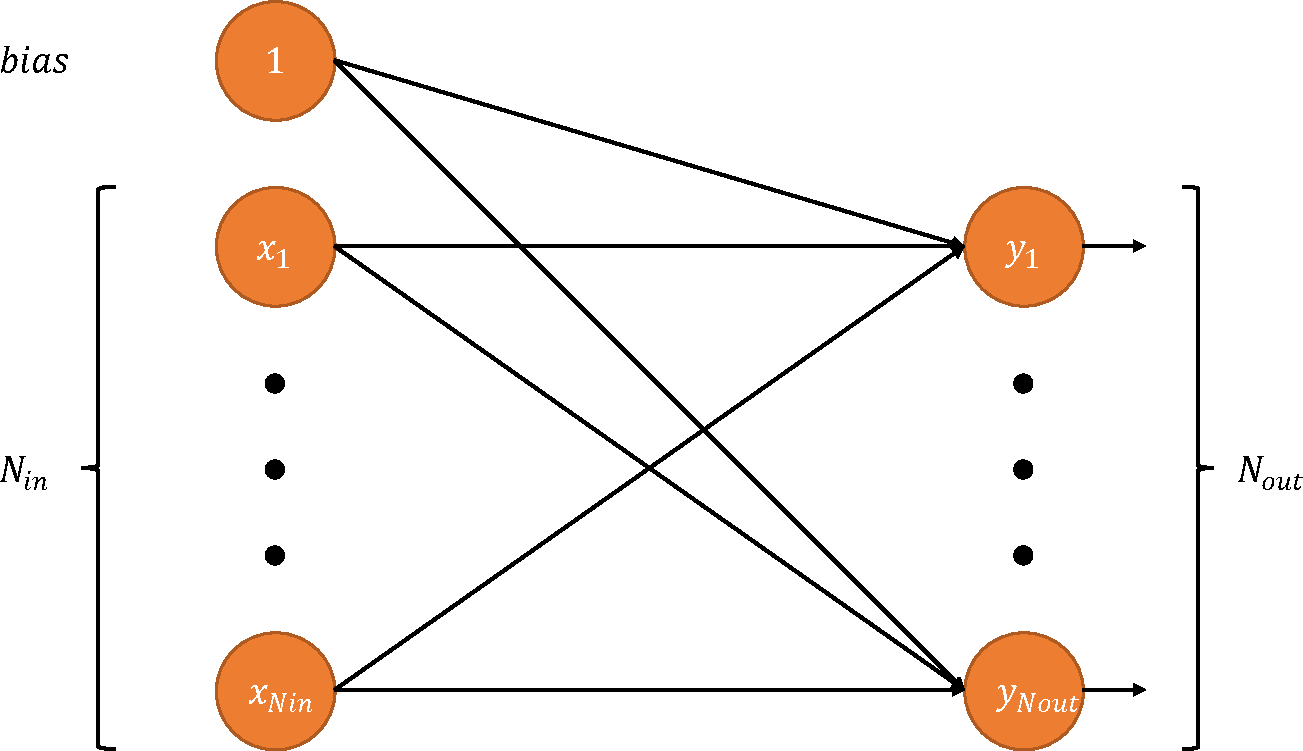
\includegraphics[width=0.9\textwidth]{fcl.pdf}
    \caption{A fully connected layer}
    \label{fig:fcn}
\end{figure}
%
A fully connected layer is characterized by the number of neurons, activation function, and the value of weights. The output vector $\boldsymbol{y}$ is defined by equation \eqref{eq:fcn}, where $\boldsymbol{x}$ is the input vector ($x_0 = 1$ corresponds to the biases), $\boldsymbol{w}$ is the weights vector ($w^i_*$ are the weights of the ith perceptron and $w^*_0$ are the biases), and $h$ is the activation function \cite{abdelouahab_accelerating_2018}.
%
\begin{equation}
    \boldsymbol{y} = h(\boldsymbol{w}^T \boldsymbol{x}) \qquad \Leftrightarrow \qquad \forall o \in \{ 1, ..., N_{out} \} : y_o = h(\sum^{N_{in}}_{i=0} w^o_i \cdot x_i)
    \label{eq:fcn}
\end{equation}
%
As we have seen that perceptrons can be used to construct a non-linear classifier, we see in next section the main operation in the \acrshort{cnn}: the \textbf{convolution}, which extracts the features from input images.